%%%%%%%%%%%%%%%%%%%%%%%%%%%%%%%%%%%%%%%%%%%%%%%%%%%%%%%%%%%%%%%%%%%%%%
% LaTeX Template: Curriculum Vitae
%
% Source: http://www.howtotex.com/
% Feel free to distribute this template, but please keep the
% referal to HowToTeX.com.
% Date: July 2011
% 
%%%%%%%%%%%%%%%%%%%%%%%%%%%%%%%%%%%%%%%%%%%%%%%%%%%%%%%%%%%%%%%%%%%%%%
% How to use writeLaTeX: 
%
% You edit the source code here on the left, and the preview on the
% right shows you the result within a few seconds.
%
% Bookmark this page and share the URL with your co-authors. They can
% edit at the same time!
%
% You can upload figures, bibliographies, custom classes and
% styles using the files menu.
%
% If you're new to LaTeX, the wikibook is a great place to start:
% http://en.wikibooks.org/wiki/LaTeX
%
%%%%%%%%%%%%%%%%%%%%%%%%%%%%%%%%%%%%%%%%%%%%%%%%%%%%%%%%%%%%%%%%%%%%%%
\documentclass[paper=a4,fontsize=11pt]{scrartcl} % KOMA-article class
							
\usepackage[english]{babel}
\usepackage[utf8x]{inputenc}
\usepackage[protrusion=true,expansion=true]{microtype}
\usepackage{amsmath,amsfonts,amsthm}     % Math packages
\usepackage{graphicx}                    % Enable pdflatex
\usepackage[svgnames]{xcolor}            % Colors by their 'svgnames'
\usepackage{geometry}
	\textheight=900px                    % Saving trees ;-)
\usepackage{url}
\usepackage{wrapfig}


\frenchspacing              % Better looking spacings after periods
\pagestyle{empty}           % No pagenumbers/headers/footers

%%% Custom sectioning (sectsty package)
%%% ------------------------------------------------------------
\usepackage{sectsty}

\sectionfont{%			            % Change font of \section command
	\usefont{OT1}{phv}{b}{n}%		% bch-b-n: CharterBT-Bold font
	\sectionrule{0pt}{0pt}{-5pt}{3pt}}

%%% Macros
%%% ------------------------------------------------------------
\newlength{\spacebox}
\settowidth{\spacebox}{8888888888}			% Box to align text
\newcommand{\sepspace}{\vspace*{0em}}		% Vertical space macro

\newcommand{\MyName}[1]{ % Name
		\Huge \usefont{OT1}{phv}{b}{n} \hfill #1
		\par \normalsize \normalfont}
		
\newcommand{\MySlogan}[1]{ % Slogan (optional)
		\large \usefont{OT1}{phv}{m}{n}\hfill \textit{#1}
		\par \normalsize \normalfont}

\newcommand{\NewPart}[1]{\section*{\uppercase{#1}}}

\newcommand{\PersonalEntry}[2]{
		\noindent\hangindent=2em\hangafter=0 % Indentation
		\parbox{\spacebox}{        % Box to align text
		\textit{#1}}		       % Entry name (birth, address, etc.)
		\hspace{1.5em} #2 \par}    % Entry value

\newcommand{\SkillsEntry}[2]{      % Same as \PersonalEntry
		\noindent\hangindent=2em\hangafter=0 % Indentation
		\parbox{\spacebox}{        % Box to align text
		\textit{#1}}			   % Entry name (birth, address, etc.)
		\hspace{1.5em} #2 \par}    % Entry value	
		
\newcommand{\EducationEntry}[4]{
		\noindent \textbf{#1} \hfill      % Study
		\colorbox{Black}{%
			\parbox{6em}{%
			\hfill\color{White}#2}} \par  % Duration
		\noindent \textit{#3} \par        % School
		\noindent\hangindent=2em\hangafter=0 \small #4 % Description
		\normalsize \par}

\newcommand{\WorkEntry}[4]{				  % Same as \EducationEntry
		\noindent \textbf{#1} \hfill      % Jobname
		\colorbox{Black}{\color{White}#2} \par  % Duration
		\noindent \textit{#3} \par              % Company
		\noindent\hangindent=2em\hangafter=0 \small #4 % Description
		\normalsize \par}

%%% Begin Document
%%% ------------------------------------------------------------
\begin{document}
% you can upload a photo and include it here...
\begin{wrapfigure}{l}{0.5\textwidth}
	\vspace*{-3em}
		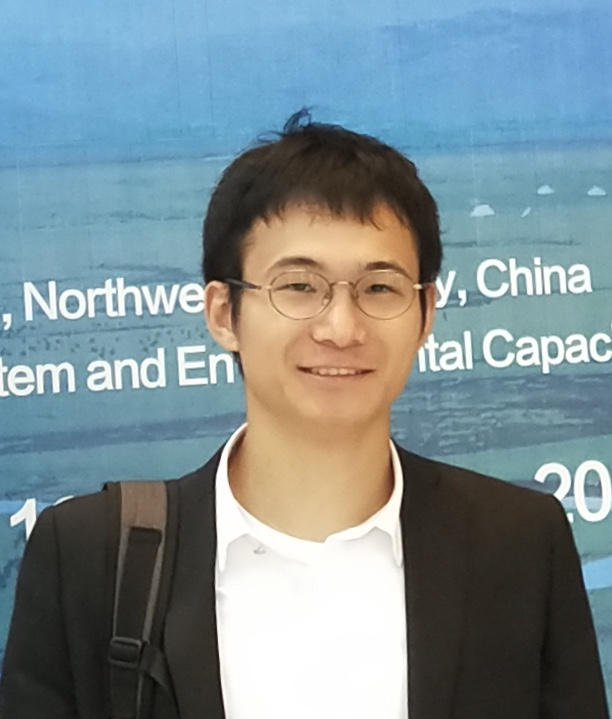
\includegraphics[width=0.15\textwidth]{./photo.jpg}
\end{wrapfigure}

\MyName{Tao Lu}
\MySlogan{Curriculum Vitae}

\sepspace

%%% Personal details
%%% ------------------------------------------------------------
\NewPart{Personal details}{}

\PersonalEntry{Birth}{January 6, 1992}
\PersonalEntry{Address}{R511 Erudorado, 2-20-23 Hashimoto}
\PersonalEntry{}{Midori Ku, Sagamihara City, Kanagawa}
\PersonalEntry{Phone}{(081) 070-2188-7509}
\PersonalEntry{Mail}{\url{uponmyword@sina.com}}

%%% Education
%%% ------------------------------------------------------------
\NewPart{Education}{}

\EducationEntry{MSc. Civil and Environmental Engineering}{2015-2017}{Chuo University Japan}{Enrolled in Program for Capacity Building in Global Water-Environmental Engineering with scholarship.}
\sepspace

\EducationEntry{BSc. Harbour,Coastal and Offshore Engineering}{2010-2014}{Hohai University China}{}

%%% Publications
%%% ------------------------------------------------------------
\NewPart{Publications}{}
Tao Lu, Tomohito Yamada, and Tadashi Yamada. "Fundamental Study of Real-time Short-term Rainfall Prediction System in Watershed: Case Study of Kinu Watershed in Japan." Procedia Engineering 154 (2016): 88-93.  

%%% Work experience
%%% ------------------------------------------------------------
\NewPart{Work experience}{}

\EducationEntry{Solution business}{2017-present}{Geosphere Environmental Technology Corporation, Full-time}{Construct 3D geological-hydrological model for various situation related to water resources and water disaster. Conduct simulation and give advice for solution.}
\sepspace


%%% Skills
%%% ------------------------------------------------------------
\NewPart{Skills}{}

\SkillsEntry{Languages}{Chinese (mother tongue)}
\SkillsEntry{}{English (fluent)}
\SkillsEntry{}{Japanese (fluent, N1)}
\SkillsEntry{}{Spanish (novice)}

\SkillsEntry{Program experience}{\textsc{Pyhton: internat worm, QGIS2.0 plugin(SuperLabeling)}}
\SkillsEntry{}{\textsc{Fortran: data processing}}
\SkillsEntry{}{\textsc{HTML: \url {https://tao4free.github.io/Hydrology/}}}


%%% Experiences
%%% ------------------------------------------------------------
\NewPart{Experiences}{}
1. Studied UCDavis(California, USA) for one month in 2016.\\
2. Attended two international conference/symposim (International Conference on Hydroinformatics (HIC 2018); ISEWS2018)

\end{document}
